\documentclass{standalone}
\usepackage{tikz}
\usepackage{ctex,siunitx,bm}
\usepackage{tkz-euclide}
\usepackage{amsmath}
\usetikzlibrary{patterns, calc}
\usetikzlibrary {decorations.pathmorphing, decorations.pathreplacing, decorations.shapes,}
\begin{document}
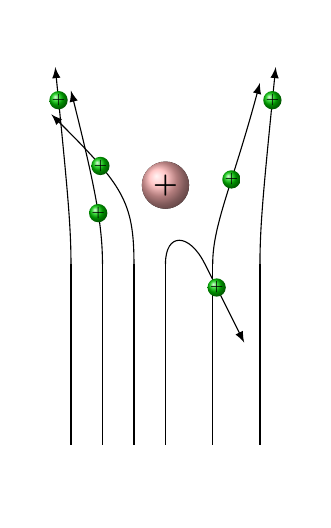
\begin{tikzpicture}[>=latex]
  \clip (-1.75,-3)rectangle(1.75,3);
  \fill[ball color=red!30](0,1)circle(3mm)node[text=black]{$\bm +$};
  \foreach \x in {-1.2,-0.8,-0.4,0,0.6,1.2}
  {
    \draw[thin](\x,-2.3)--(\x,0);
  }
  \draw[thin,->](-1.2,0)..controls(-1.2,0.5)and(-1.25,1)..(-1.4,2.5)
    node[pos=0.9,ball color=green!80!black,circle,inner sep=0pt]{\tiny$+$};
  \draw[thin,->](1.2,0)..controls(1.2,0.5)and(1.25,1)..(1.4,2.5)
    node[pos=0.9,ball color=green!80!black,circle,inner sep=0pt]{\tiny$+$};
  \draw[thin,->](-0.8,0)..controls(-0.8,0.5)and(-0.9,1)..(-1.2,2.2)
    node[pos=0.4,ball color=green!80!black,circle,inner sep=0pt]{\tiny$+$};
  \draw[thin,->](0.6,0)..controls(0.6,0.5)and(0.85,1)..(1.2,2.3)
    node[pos=0.6,ball color=green!80!black,circle,inner sep=0pt]{\tiny$+$};
  \draw[thin,->](-0.4,0)..controls(-0.4,0.8)and(-0.55,1.0)..(-1.45,1.9)
    node[pos=0.7,ball color=green!80!black,circle,inner sep=0pt]{\tiny$+$};
    \draw[thin,->](0,0)..controls(0,0.4)and(0.3,0.4)..(0.5,0)--(1,-1)
    node[pos=0.3,ball color=green!80!black,circle,inner sep=0pt]{\tiny$+$};
\end{tikzpicture}
\end{document}